\section{Свойства и графики степенной функции}

\begin{definition}
    Степенная функция -- функция вида $f(x) = x^n$
\end{definition}

\subsection{Натуральная нечетная степень}

$f(x) = x^n, \; n \in \mathbb{N}  \land n \notdivisible 2$

\begin{itemize}
    \item $D(f) = \mathbb{R}$
    можем подставить любое число
    \item $E(f) = \mathbb{R}$
    согласно теореме \hyperref[thm:1.2.3]{о корректности определения}
    \item $f \uparrow \mathbb{R}$\\
    \begin{align*}
        &\forall x_1, x_2 : x_1 > x_2 \\
        &f(x_1) - f(x_2) = x_1^n - x_2^n = \underbrace{(x_1 - x_2)}_{> 0} \underbrace{(x_1^{n-1} + x_1^{n-2}x_2 + x_1^{n-3}x_2^2 \; \dots \; x_1x_2^{n-2} + x_2^{n-1})}_{> 0 \text{ см. ниже}} \\
    \end{align*}
    1. $x_1 > x_2 \ge 0$ - очевидно \\
    2. $x_1 > 0 > x_2$ - очевидно, $x_1^n - x_2^n > 0$ \\
    3. $0 \ge x_1 > x_2$ - см. четность степеней \\ \\
    Тогда
    \begin{align*}
        f(x_1) - f(x_2) > 0 \Rightarrow f(x_1) > f(x_2)
    \end{align*}
\end{itemize}

\begin{remark}
    С ростом $n$ график стремится к <<качерге>>, круто падая до $-1$ и круто растя после $1$
\end{remark}

\newpage

\begin{figure}[h]
    \centering
    \begin{subfigure}{0.35\textwidth}
        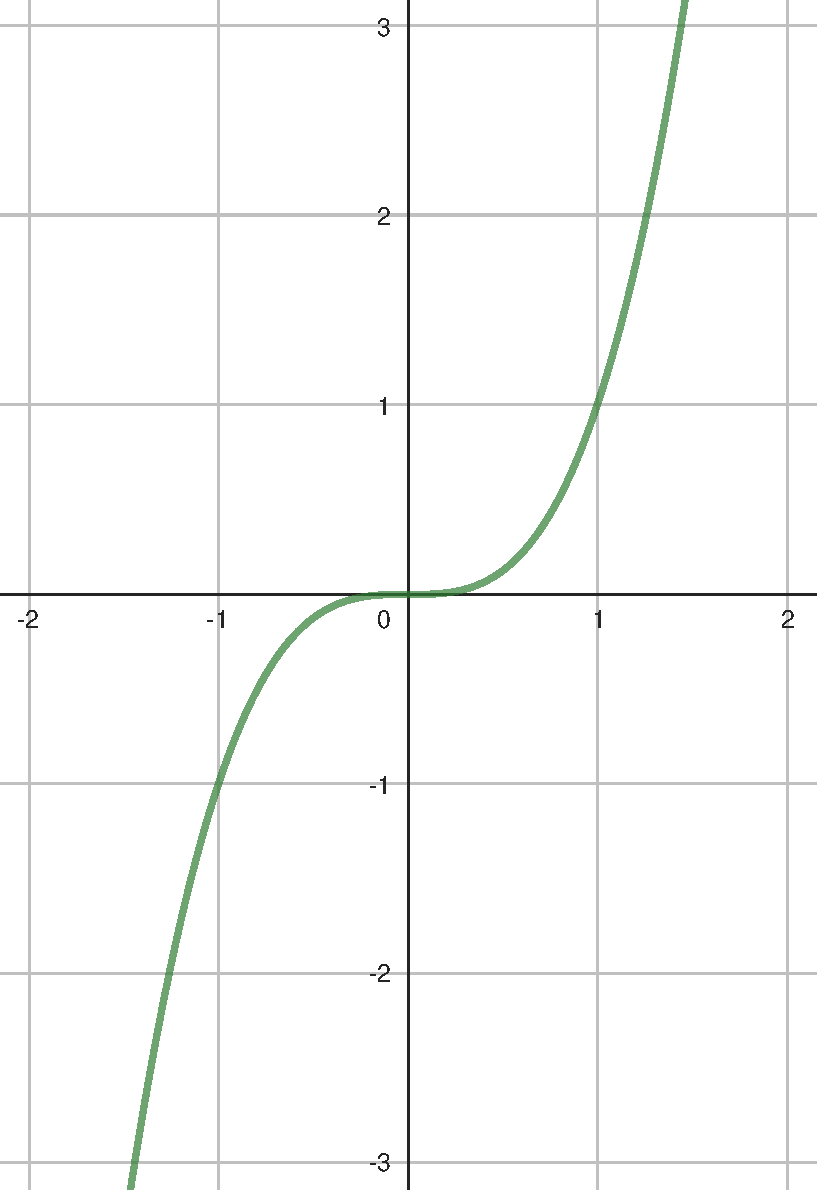
\includegraphics[width=\textwidth]{tex/chapter_1/assets/y=x^3.pdf}
        \caption*{$f(x) = x^3$}
    \end{subfigure}
    \hfill
    \begin{subfigure}{0.35\textwidth}
        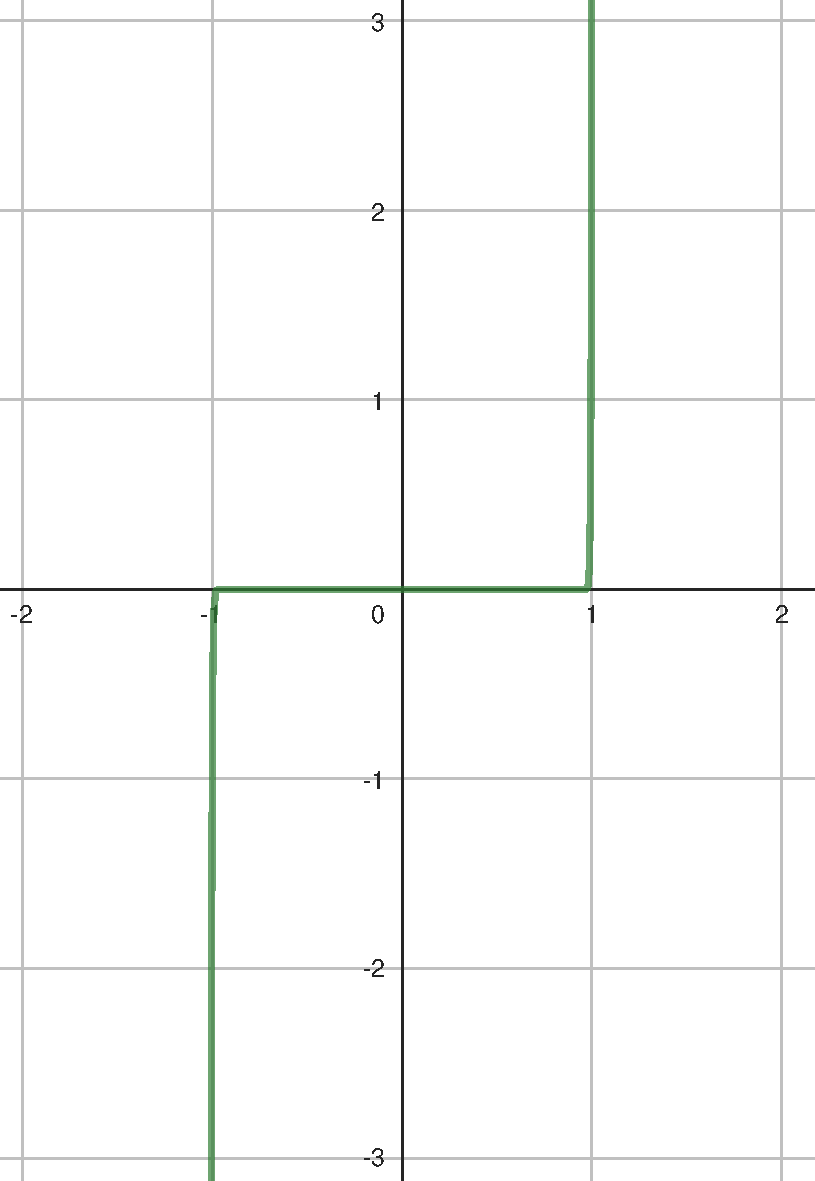
\includegraphics[width=\textwidth]{tex/chapter_1/assets/y=x^239.pdf}
        \caption*{$f(x) = x^{239}$}
    \end{subfigure}
\end{figure}


\subsection{Натуральная четная степень}

$f(x) = x^n, \; n \in \mathbb{N}  \land n \divisible 2$

\begin{itemize}
    \item $D(f) = \mathbb{R}$
    можем подставить любое число
    \item $E(f) = [0;+\infty)$
    согласно теореме \hyperref[thm:1.2.2]{о корректности определения}
    \item $f \uparrow [0;+\infty) \land f \downarrow (-\infty; 0]$
    \begin{align*}
        &\forall x_1, x_2 : x_1 > x_2 \\
        &f(x_1) - f(x_2) = x_1^n - x_2^n = \underbrace{(x_1 - x_2)}_{> 0} \underbrace{(x_1^{n-1} + x_1^{n-2}x_2 + x_1^{n-3}x_2^2 \; \dots \; x_1x_2^{n-2} + x_2^{n-1})}_{(*)} \\
    \end{align*}
    1. $x_1 > x_2 \ge 0 \Rightarrow (*) > 0$ - очевидно \\
    2. $ 0 \ge x_1 > x_2 \Rightarrow (*) < 0$ - см. четность степеней \\ \\
    Тогда
    \begin{align*}
        &\forall x_1, x_2 \in [0; +\infty) \land x_1 > x_2 \\
        &f(x_1) - f(x_2) > 0 \Rightarrow f(x_1) > f(x_2) \Rightarrow f \uparrow [0; +\infty) \\ \\
        &\forall x_1, x_2 \in (-\infty; 0] \land x_1 > x_2 \\
        &f(x_1) - f(x_2) < 0 \Rightarrow f(x_1) < f(x_2) \Rightarrow f \downarrow (-\infty; 0]
    \end{align*}
\end{itemize}

\begin{remark}
    При росте $n$ график будет стремится к перевернутой букве <<п>>
\end{remark}

\newpage

\begin{figure}[h]
    \centering
    \begin{subfigure}{0.35\textwidth}
        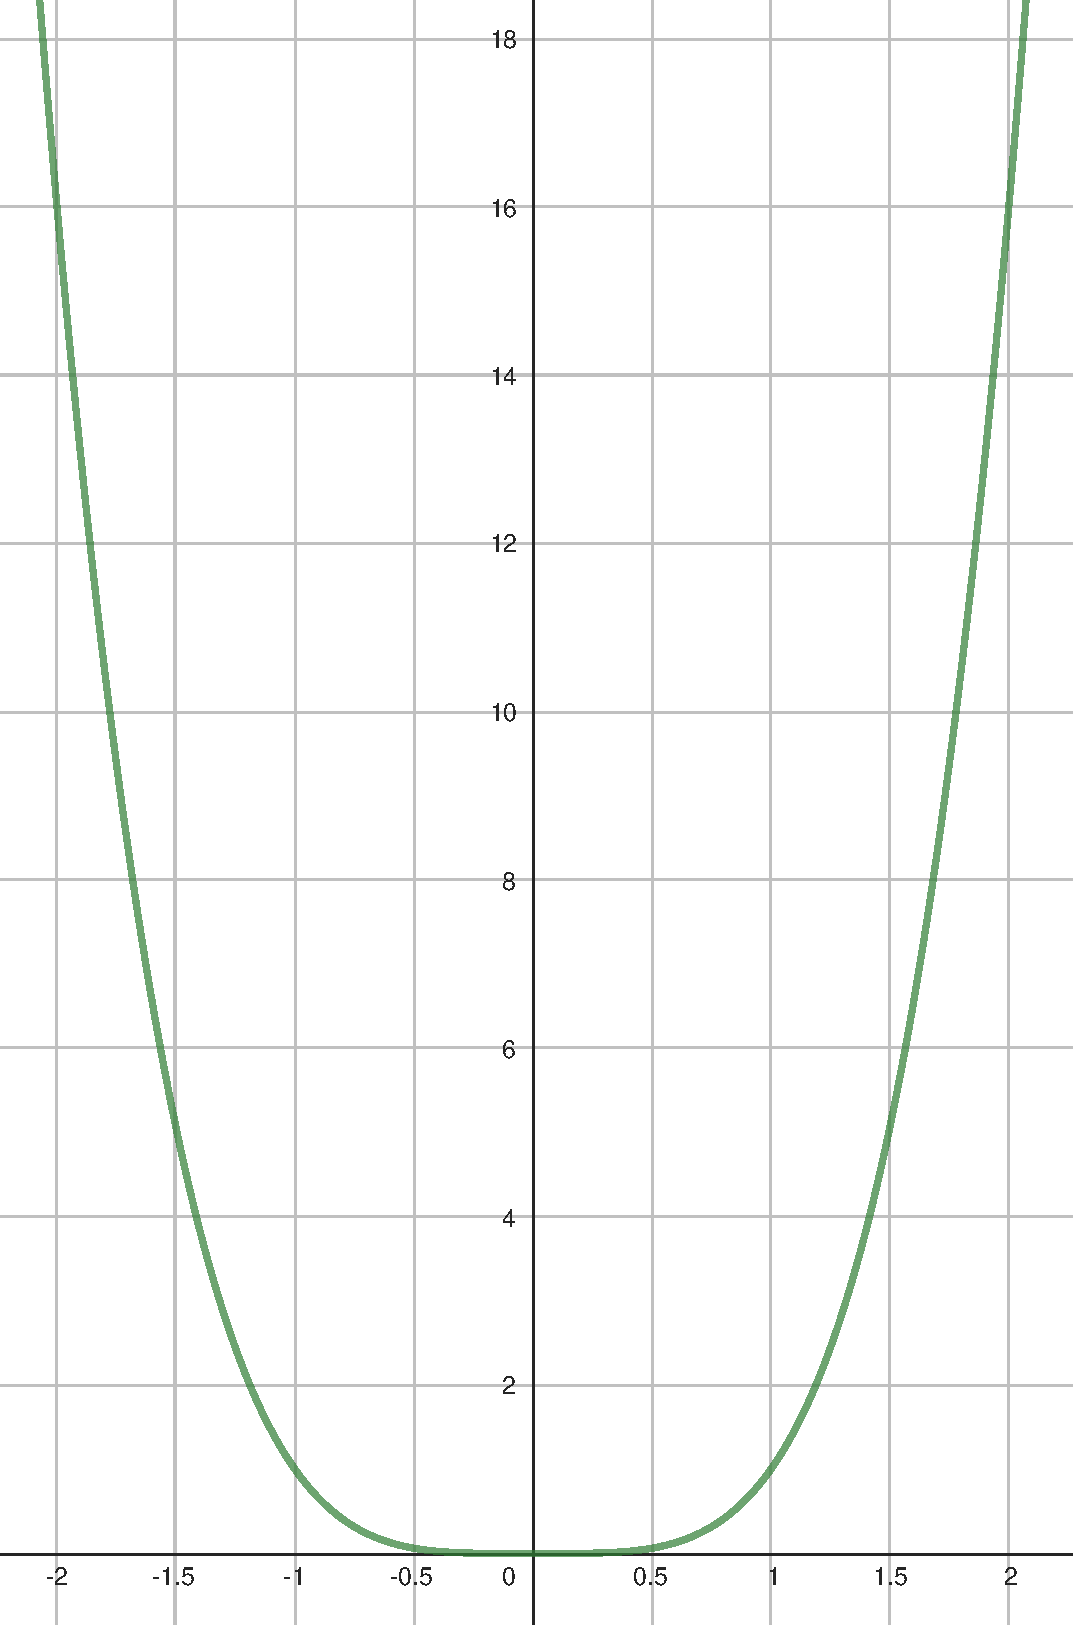
\includegraphics[width=\textwidth]{tex/chapter_1/assets/y=x^4.pdf}
        \caption*{$f(x) = x^4$}
    \end{subfigure}
    \hfill
    \begin{subfigure}{0.35\textwidth}
        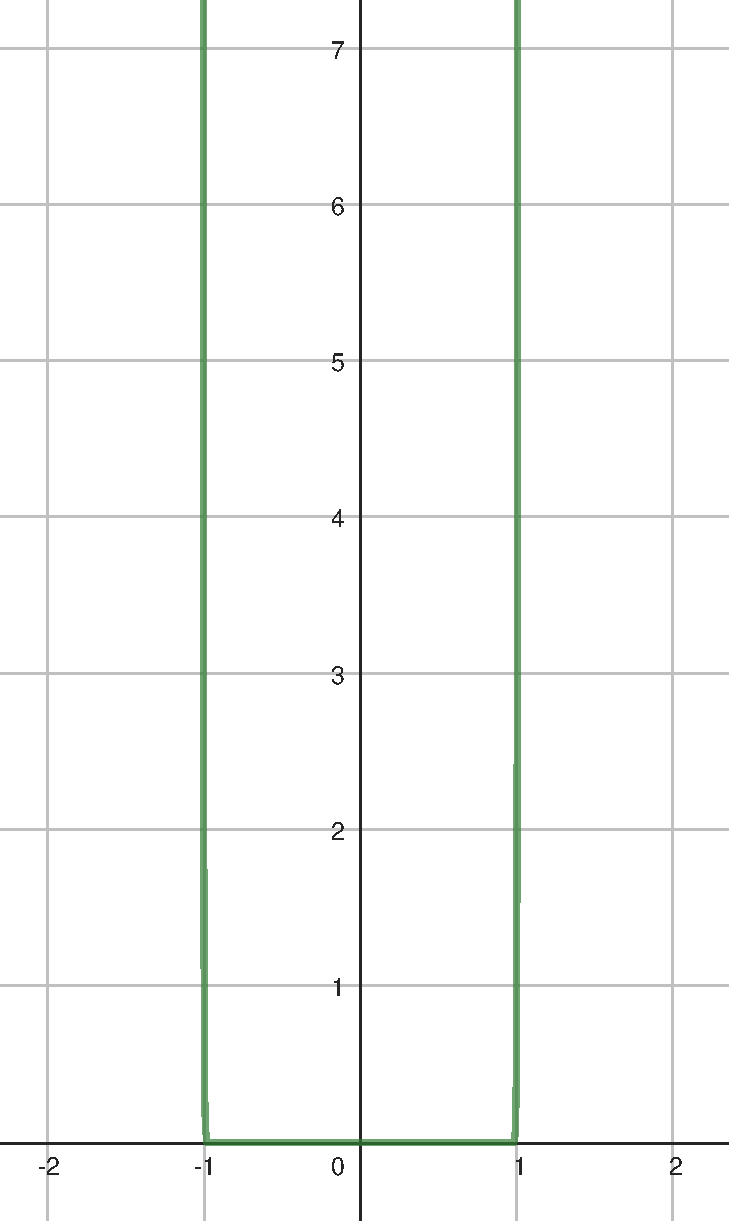
\includegraphics[width=\textwidth]{tex/chapter_1/assets/y=x^300.pdf}
        \caption*{$f(x) = x^{300}$}
    \end{subfigure}
\end{figure}

\subsection{Привет, это Гипербола}

$f(x) = x^m, \; m \in \mathbb{Z} \land m < 0 \land m \notdivisible 2 \iff f(x) = \frac{1}{x^n}, \; n = -m \land n \in \mathbb{N} \land n \notdivisible 2$ \\

\begin{itemize}
    \item $D(f) = \mathbb{R} \backslash \{0\}$
    на ноль делить нельзя
    \item $E(f) = \mathbb{R} \backslash \{0\}$
    уравнение $y = \frac{1}{x^n}$ имеет решения только при $x \neq 0$ 
    \item $f \downarrow (-\infty; 0) \land f \downarrow (0; +\infty)$
    \begin{align*}
        &\forall x_1, x_2 : x_1 > x_2 \\
        &f(x_1) - f(x_2) = \frac{1}{x_1^n} - \frac{1}{x_2^n} = \frac{x_2 - x_1}{x_1x_2}\\
    \end{align*}
    Тогда
    \begin{align*}
        &\forall x_1, x_2 \in (0; +\infty) \land x_1 > x_2 \\
        &f(x_1) < f(x_2) \Rightarrow f \downarrow (0; +\infty) \\ \\
        &\forall x_1, x_2 \in (-\infty; 0) \land x_1 > x_2 \\
        &f(x_1) < f(x_2) \Rightarrow f \downarrow (-\infty; 0) \\ \\
    \end{align*}
\end{itemize}

\begin{remark}
    Неверно, что $f \downarrow (-\infty; 0) \cup (0; +\infty)$
\end{remark}

\begin{remark}
    С ростом $n$ (и, соотвеетственно с уменьшением $m$) график будет стремится к двум кочергам в первой и третьей четверти плоскости.
\end{remark}

\begin{figure}[h]
    \centering
    \begin{subfigure}{0.35\textwidth}
        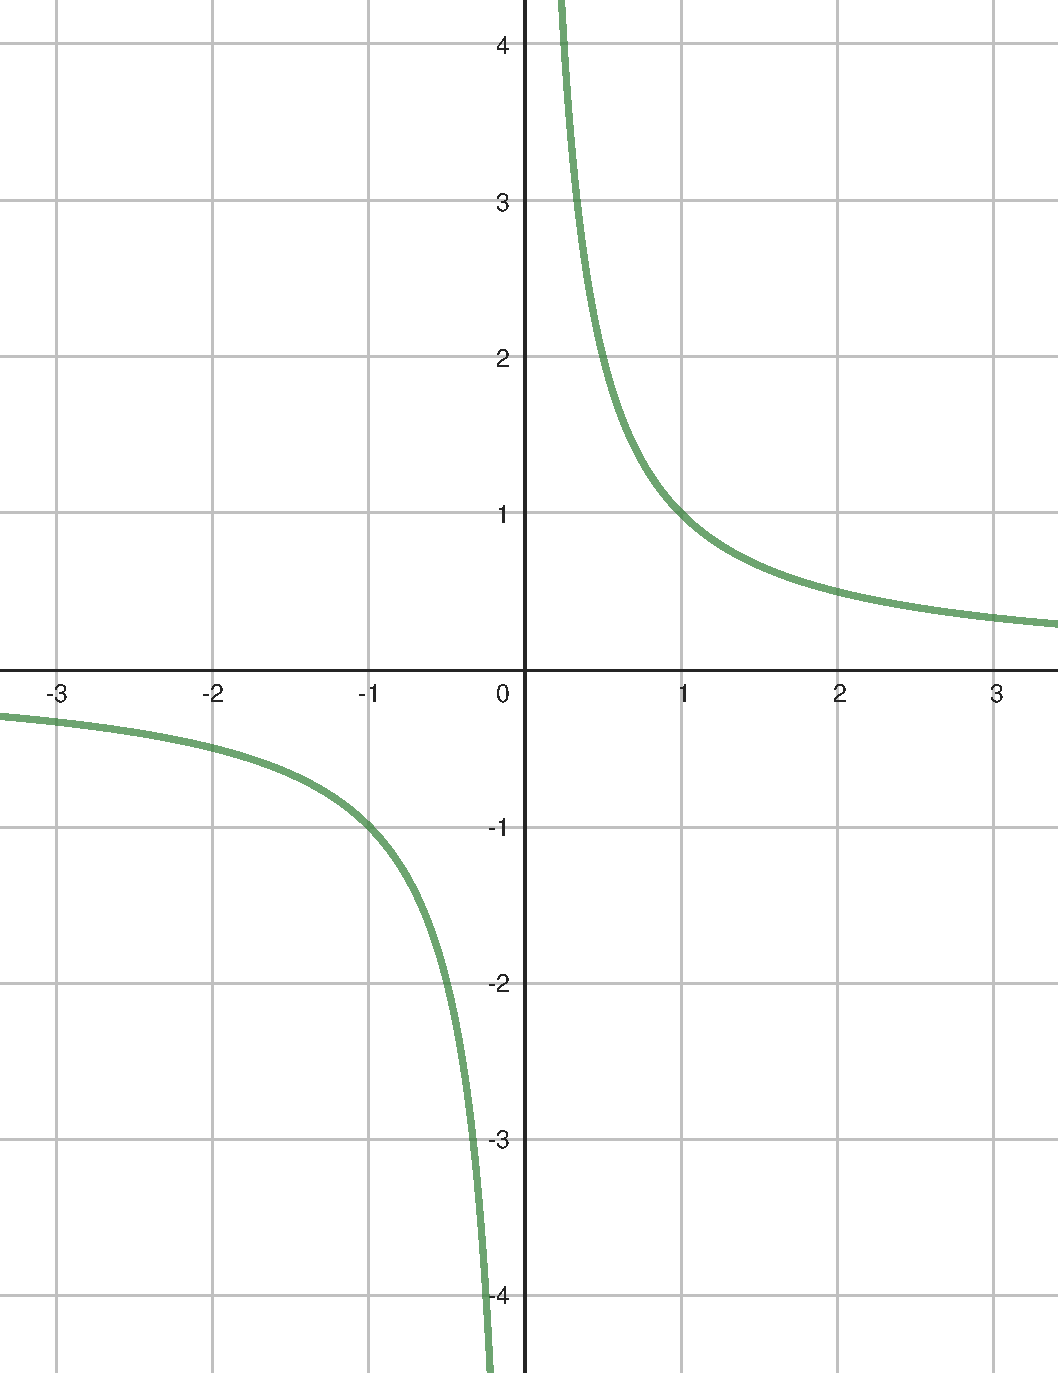
\includegraphics[width=\textwidth]{tex/chapter_1/assets/y=1_div_by_x.pdf}
        \caption*{Гипербола, $f(x) = \frac{1}{x}$}
    \end{subfigure}
    \hfill
    \begin{subfigure}{0.35\textwidth}
        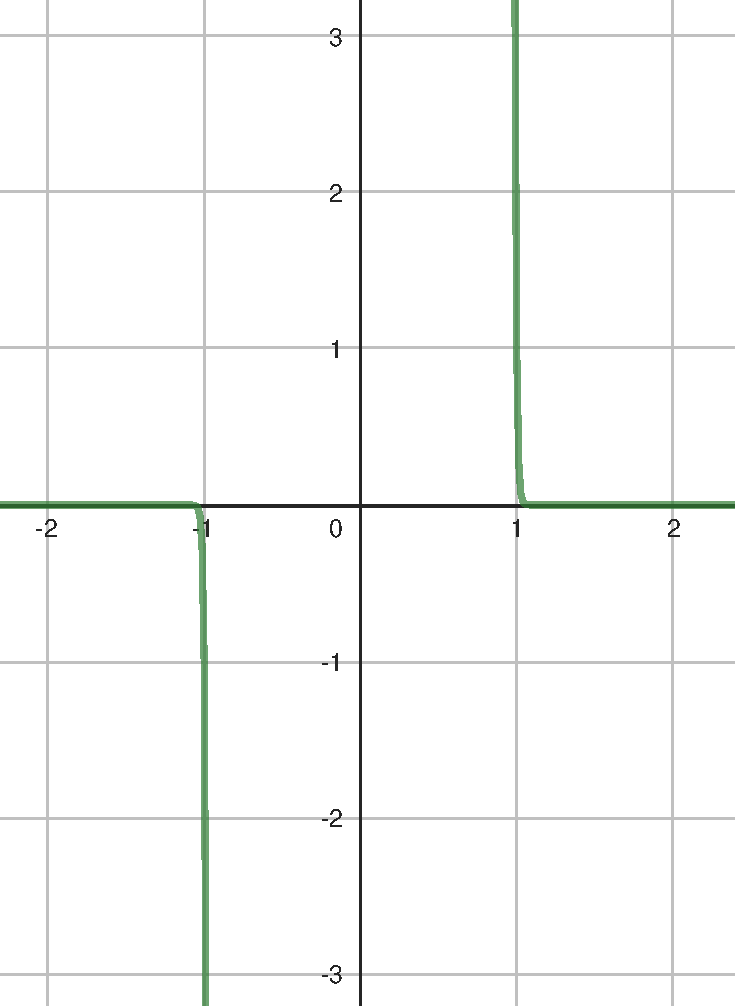
\includegraphics[width=\textwidth]{tex/chapter_1/assets/y=1_div_by_x^99.pdf}
        \caption*{$f(x) = \frac{1}{x^{99}}$, не гипербола}
    \end{subfigure}
\end{figure}

\begin{remark}
    Гиперболой называется график функции $f(x) = \frac{1}{x}$. Другие графики функций вида $f(x) = \frac{1}{x^n}$ не являются гиперболой.
\end{remark}